\documentclass[12pt]{article}
\usepackage{amsmath}
\usepackage{float}
\usepackage{amsthm}
\usepackage[psamsfonts]{amssymb}
\usepackage{graphics,epsfig}
\usepackage{enumitem}
\usepackage{hyperref}

\usepackage[sort&compress,numbers,square]{natbib}
\bibliographystyle{plainnat}

\title{Bayesian Additive Regression Networks}

\author{Daniel Van Boxel}
\date{\today}

\usepackage{xcolor}
\newcommand{\dvb}[1]{\textcolor{blue}{DVB: #1}}
\newcommand{\crp}[1]{\textcolor{olive}{CRP: #1}}

\begin{document}
\maketitle

\begin{abstract}

    We apply Bayesian Additive Regression Tree (BART) principles to training an ensemble of small neural networks for regression tasks.  Using Markov Chain Monte Carlo, Bayesian Additive Regression Trees (BARN) samples from the space of single hidden layer neural networks that are conditioned on their fit to data.  To create an ensemble of these, we apply Gibbs' sampling to update each network against the residual target value (i.e. subtracting the effect of the other networks).  We examine the effectiveness of BARN on several benchmark regression tasks, comparing it to equivalent neuron count single neural networks as well as equivalent tree count BART.  We also apply BARN to a more recent modeling problem and compare with state of the art.  Our Bayesian Additive Regression Networks (BARN) provide more consistent and often more accurate results, at the cost of significantly greater computation time.  BARN seems to perform best on problems with modest data and significant nonlinearity, though this needs further study.  It is highly adaptable, performing well on a variety of problems.
\end{abstract}

\section{Introduction}\label{sec:intro}

Training a cooperative set of weak models (i.e. an ensemble of small models) rather than a single large model has proven itself an effective machine learning technique \cite{dietterich2000ensemble,hansen1990neural,seni2010ensemble,lee2020comparing}.  While Random Forests (RF) \cite{ho1995random,breiman2001random} are one of the most well-known ensemble methods, multiple other approaches have been proposed over the years, \cite[provide some reviews]{way2012advances,dong2020survey}.  One tree-based technique that has outperformed more recent models \cite{biau2019neural} is Bayesian Additive Regression Trees (BART) \cite{chipman2010bart}.  At the same time, neural networks (NNs) have become extremely accurate on a wide variety of tasks \cite{schmidhuber2015deep}, attracting attention from more traditional machine learning methods.

Seeking even better methods, some researchers have attempted to combine tree-based and NN-based approaches.  For instance, Neural Random Forests \cite{biau2019neural}, builds NNs that are numerically equivalent to RFs, and then continues to train them as though they were newly initialized networks.  Recent research \cite{vanboxel2021neural}, however, suggests creating neural networks this way may not significantly improve performance over both similarly parametrized RFs and NNs.  Another attempted hybridization is Neural Decision Trees \cite{balestriero2017neural}, which replaces the splitting function in trees with neural networks.

Rather than copy an existing ensembling approach exactly into neural networks \cite[for example]{biau2019neural}, we instead adapt the conditional Monte Carlo Markov Chain (MCMC) learning process of BART \cite{chipman2010bart} to an ensemble of neural network architectures.  That is, we train a series of NNs, each one on the residual of the target value and the summed prediction of the remaining NNs.  We further condition acceptance of a model following the Bayes CART method \cite{chipman1998bayesian}.  This sampling procedure of Bayesian Additive Regression Networks (BARN) generalizes the BART method to a new model type.  We describe this in more detail in \autoref{sec:method}.

To evaluate the effectiveness of this approach, we apply BARN to a variety of benchmark data sets \cite{Dua:2019} as used in the Neural Random Forests \cite{biau2019neural} study.  We also examine a more recent ecological data set \cite{roman2022bayclump}.  To limit computation time, we restrict our analysis to prototype size (mean 4 neurons) and number networks (fixed at 10) in the ensemble.  We additionally train, however, equivalent sized (to the entire ensemble) NNs and equivalent-count BART forests (i.e. 10 decision trees) for comparison.  We find that BARN, though expensive (in its current implementation), is able to reliably match or beat performance of both alternatives.  It is robust to different modeling problems, even when it does not produce the most accurate result, it was always close, and never the worst performing model.

\section{Related Work}\label{sec:related}

\emph{MCMC:} Before discussing machine learning techniques, we briefly describe some key works in MCMC that allow us to intelligently sample from the space of \emph{models} (which may or may not include learned model parameters).  Metropolis et al \cite{metropolis1953equation} developed one of the earliest MCMC algorithms to sample from a target distribution, enabling sampling without direct simulation.  Hastings \cite{hastings1970monte}, however, provided a key extension (hence why this process is sometimes called the ``Metropolis-Hastings'', or M-H, algorithm) to allow transition probabilities to vary in direction (i.e. the probability of transiting from the initial state to the proposed state need not be equal to the probability of transiting from the proposed state to the initial state).  Though a special case of M-H, Gibbs Sampling \cite{geman1984stochastic} demonstrated a way to iteratively update components of a model.  More recently, Green \cite{green1995reversible} introduced Reversible-Jump MCMC to handle situations when the dimension size of the state space may change (i.e. when transiting the space of models rather than continuous values).  Finally, Hastie and Tibshirani \cite{hastie2000bayesian} synthesized these into a method for fitting a statistical \emph{model}, applying sampling techniques beyond the data itself.

\emph{BART:} One such statistical model is BART, part of a long line of machine learning methods focused on decision trees.   A decision tree is a formalization of the principle of following a sequence of queries to a single result that has long existed in fields like phylogenetics (often called, ``dichotomous keys'') for classifying species \cite{pankhurst1991practical}.  In machine learning, however, researchers have developed methods to build optimal trees for both classification (e.g. ``Commute by bus, car, or train?'') and regression \cite{breiman1984classification} (e.g. ``What's the fuel efficiency of a car?'').  In particular, Bayesian Classification And Regression Trees (CART) \cite{chipman1998bayesian} uses Markov Chain Monte Carlo to sample from the \emph{space of trees}, conditioned on how well the proposed tree models the data (See \autoref{sec:background} for additional details).  BART \cite{chipman2010bart} then extends the CART procedure to a sum-of-models ensemble (i.e. the ``additive'' part of BART) by using Gibbs Sampling, providing state-of-the-art regression modeling using simple decision trees. 

\emph{NN:} Another arguably state-of-the-art approach in machine learning is neural networks (NNs).  In recent decades, NNs have come to prominence for their accuracy and ease-of-use \cite{schmidhuber2015deep}.  Starting from the Perceptron \cite{rosenblatt1958perceptron}, neural networks are now routine in computer vision \cite{tan2019efficientnet}, regression, and classification.  Often, the challenge in training an NN (beyond managing large volumes of data) is determining the network architecture itself.  Idrissi et al \cite{idrissi2016genetic} proposed a genetic algorithm for search, though this can be computationally expensive.  Zoph and Le \cite{zoph2016neural} as well as Liu et al \cite{liu2018progressive} investigated iterative approaches to build up a network.  Coming from the other direction of pruning, Lecun et al \cite{lecun1989optimal} was an early work at minimizing the set of required connections.  Architecture search is still often regarded as an art-form more than an optimization.

\emph{Bayesian Modeling}: Taking a Bayesian approach to modeling means putting prior distribution on model parameters.  These priors usually derive from earlier studies, physical models, or system constraints.  Sometimes the priors are internal to the study, as in one traffic safety model \cite{schneider2009bayesian}, while others use priors from previous work \cite{roman2022bayclump}.  Regardless, these affect final estimated parameter results through the classic Bayes' formula \cite{johnson2022bayes}.

\emph{Ensemble Models:} Though neural networks and other solitary large models can be effective, some studies have shown greater capability in an \emph{ensemble} of smaller (i.e. individually less accurate) models \cite{hastie2009elements}.  Random Forests \cite{breiman1996bagging} are a direct approach to this, essentially averaging the result of many small decision trees.  Biau et al \cite{biau2019neural} devised Neural Random Forests to create a (single) neural network from such a forest, with mixed results.  Though a sum-of-models, BART itself is a forest (i.e. ensemble) of decision trees \cite{chipman2010bart}.  To ensemble NNs instead, Opitz and Shavlik \cite{opitz1996actively} used a genetic algorithm to find diverse candidates.  But this doesn't take advantage of conditional statistics demonstrated in BART, which we adapt.

\section{Background}\label{sec:background}


To understand the technique we develop to train an ensemble of neural networks (BARN), we first detail some of the core components to the method.  While many specifics (e.g. full Monte Carlo theory, supporting model assumptions, etc) are beyond the scope of this paper, we intend to convey the necessary basics of machine learning and the M-H algorithm.

While machine learning takes many forms, we focus on neural networks to model regression problems.  For a given data point, we model each target value, $y \in \mathbb{R}$ as some function of independent variables, $x \in \mathbb{R}^n$, such that for each data point $x_i$, we have some error term, $\epsilon_i$, and $y_i$.

$$
y_i = f(x_i) + \epsilon_i
$$

In ordinary linear regression (OLS), we have a linear function $f(x_i) = \sum_j w_j x_{ij}$ (where $x_{ij}$ is the $j$th variable of the $i$th data point), and we assume the error terms ($\epsilon_i$) are normally distributed.  If the target really is a linear function of the input variables plus some noise (and a few other mild assumptions), this can be a very accurate model.  But this approach may fail if the true model is something nonlinear (e.g. $y_i = 2x_{i1} + 3x_{i2}^2 + \epsilon_i$).  We would need a nonlinear component in our model to accurately capture the nonlinear term in the data (e.g. generating a new $x_{i3} =x_{i2}^2$).

Neural networks provide a very general nonlinear structure and train weights to model precisely these kinds of behaviors \cite{hastie2009elements}.  First, we construct a single ``neuron'',

$$
h_k(x_i) = g(\sum_j w_j x_{ij})
$$

where $w_j$ is some trainable parameter, and $g$ is a nonlinear ``activation'' function.  We can create many neurons (e.g. $h_1, h_2, h_3$) based on the same input $x$ using different sets of weights $w_j$ (sometimes denoted $w_J^k$ for indexing).  Thus each $h_k$ represents a different nonlinear function of the input.  We refer to this set of neurons as a ``hidden layer''.  Next, we can ether apply an OLS to the neuron outputs to model $y$, or we can construct another layer using the outputs of the previous layer (i.e. using $h_k$ values rather than $x$ values directly).  \autoref{fig:nn} shows an example layout of a single hidden layer neural network.  $x$ values are inputs into the $h_k$ functions of the hidden layer.  And a weighted sum of $h_k$ values  (i.e. OLS) predicts the target $y$ value, completing the NN calculation.

\begin{figure}[htb]
\centering
    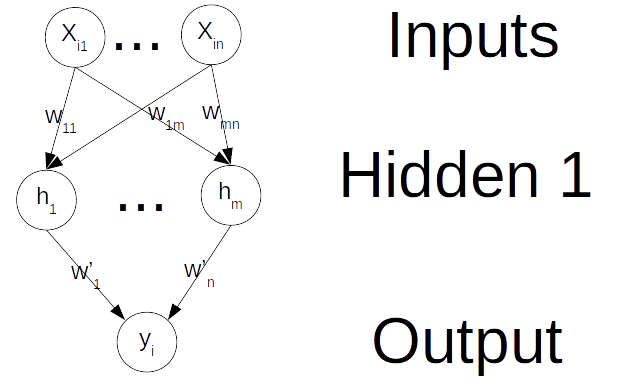
\includegraphics[scale=1]{nn.png}
    \caption{Single hidden layer neural network predicts $y \in \mathbb{R}$ as a generic nonlinear function of $x \in \mathbb{R}^n$.  Note non-numeric input variables must be encoded numerically (e.g. as indicator variables).}
    \label{fig:nn}
\end{figure}

Though this specifies the \emph{architecture} of the NN, but we still need to determine the values of all the $w$ weights.  Determining the values of $w$ is an optimization problem for which one can apply many methods.  Some common approaches are gradient-based backpropagation such as Adam \cite{kingma2014adam} or stochastic gradient descent \cite{hastie2009elements}.  The details are not critical to our analysis; only that our network activation functions be almost everywhere differentiable so that we can compute gradients.

We also briefly note that we can create an ensemble of models like NNs in an ``additive'' way.  Let $f_1, f_2, \cdots, f_N$ be $N$ different NNs all operating on the same input $x$ and producing one output each.  Note that we fix the number of NNs just as BART fixes the number of trees \cite{chipman2010bart}.  Now let model $\hat{y}_i = \sum_j f_j(x_i)$ so that $\hat{y}_i \approx y_i$.  We use this additive form rather than averaging (i.e. $\hat{y}_i = \frac{1}{N} \sum_j f_j(x_i)$, though this only differs by a constant scaling factor) so that we can train individual NNs on the residual of the target and the remaining NN contributors, similar to BART \cite{chipman2010bart}.  That is, we will train network $i$ by first fixing all of the other networks in the ensemble.  Then we subtract their fixed contribution to the estimate from the actual target value to produce a residual.  We train the free network on the residual defined as follows:

$$
R_{ik} = y_i - \sum_{j\neq k} f_j(x_i)
$$

To develop our ensemble of NNs, we sample from the space of networks using a Markov Chain.  In a simple MCMC procedure, we would sample from some target distribution, $P(x)$, that is, in general, difficult to sample from directly \cite{haugh2021tutorial}.  To do this sampling, we construct a Markov Chain whose stationary distribution is $P(x)$.  One straightforward way to ensure this is make sure the probability flux from state $x$ to state $x'$ in our procedure is equal to the probability flux of moving from state $x'$ to $x$, shown in \autoref{fig:balance}.  This is known as enforcing ``detailed balance''.

\begin{figure}[htb]
\centering
    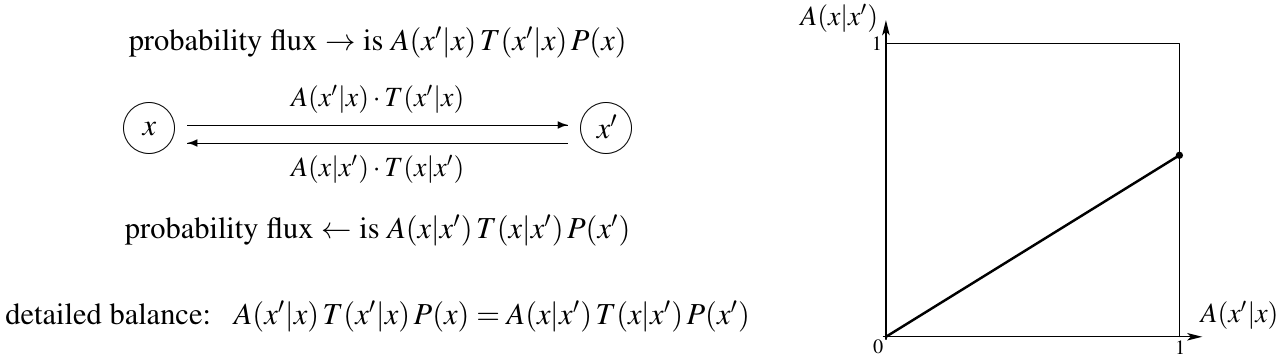
\includegraphics[scale=0.4]{balance.png}
    \caption{Share of probability from $x$ moving to $x'$ is equal to share from $x'$ moving to $x$ for all pairs of states, ensuring overall distribution is constant.  Figure reproduced from \cite{stepanov2021math}.}
    \label{fig:balance}
\end{figure}

There are several terms in this detailed balance description in \autoref{fig:balance}.  $A(x,x')$ is the acceptance probability of moving to the new state $x'$ from $x$, and $T(x,x')$ is the underlying transition probability of state $x$ changing to state $x'$.  The MCMC procedure starts from some initial $x$ state (say $x=0$ in a simple 1D continuous case), proposes a new state, $x'$, and then accepts it with some probability:

$$
A(x,x') = min(1, \frac{T(x|x') P(x')}{T(x'|x) P(x)})
$$

Intuitively, if we propose a ``more likely'' state ($P(x') \geq P(x)$) and it's at least as likely to transit from $x'$ to $x$ as the other way ($T(x|x') \geq T(x'|x)$), then we will accept the new state with probability 1.  If either of these conditions fails, there is only some chance (possibly still probability 1), depending on the exact values, of accepting the new state \cite{stepanov2021math}.  Note that if we were reject every less likely state, we would lose detailed balance and no longer have the desired stationary distribution.  After a number of ``burn-in'' iterations, the distribution of states over time converges to the desired $P(x)$.  Note, however, that successive times are necessarily correlated.

For BART and BARN, however, we sample not from a known distribution, but from the distribution of models that accurately predict our target value (i.e. smaller residuals).  Consider a generic model, $M$ (e.g. a decision tree or a neural network).  Generalizing the bayesian CART procedure \cite{chipman1998bayesian}, we expand the target distribution into two components: 

$$
P(x) = P(Y|X,M) P(M)
$$

where $P(M)$ is some Bayesian prior on the model itself, independent of the data.  We typically use this prior to control model size (e.g. encourage smaller models).  On the other hand, $P(Y|X,M)$ represents how well the model fits the data (target $Y$ with input $X$).  Our transition probabilities (in BARN or BART), $T(M,M')$ have some specification as well (note that this mostly affects the efficiency and speed of convergence of the procedure).  Our revised conditional acceptance is then:

$$
A(M,M') = min(1, \frac{T(M|M') P(Y|X,M')P(M')}{T(M'|M) P(Y|X,M)P(M)})
$$

This acceptance probability still only applies to a single model, not an ensemble as in BART or BARN.  Transitioning $n$ such models at once is cumbersome, requiring an $n^2$ transition dimension \emph{in the space of models, $M$,} and a similarly complicated conditional.  Instead, BARN applies Gibbs Sampling to iteratively update models based on the residual, exactly as is done in BART \cite{chipman2010bart}.  short, this means that when updating model $M_k$, we first compute the residual with the other models, $R_k$.  Then we take one MCMC step with acceptance:

$$
A(M_k,M_k') = min(1, \frac{T(M_k|M_k') P(R_k|X,M_k')P(M_k')}{T(M_k'|M_k) P(R_k|X,M_k)P(M_k)})
$$

When we update the $M_{k+1}$ model, we recompute the residual using the possibly new $M_k$.  This allows us to quickly update each model's contribution and maintain the overall MCMC procedure.  As in BART, this MCMC prodcedure converges to an ensemble of models conditioned on their ability to additively predict the target.

\section{Methodology}\label{sec:method}

We adapt the BART procedure \cite{chipman2010bart} to an ensemble of small single-hidden layer neural networks instead of decision trees.  That is, we train the ensemble such that $\hat{y}_i = \sum_k M_k(x_i)$, where each $M_k$ is a neural network with some number of neurons and one hidden layer.  In principle the model can be arbitrarily more complicated, but we retain this structure to simplify MCMC calculations and reduce computation time.  Due to the similarities with BART, we call our procedure Bayesian Additive Regression Networks (BARN).

At a high level, we propose architectural changes to a single model, $M_k$, at a time.  This single model changes enable us to condition on the fixed models, $M_{j\neq k}$ to effect Gibbs' sampling.  Each MCMC step proposes a modification to $M_k$'s architecture, trains this new model, and computes an acceptance probability, $A$.  For simplicity, we fix the \emph{number} of models in the ensemble as $N$.  The MCMC procedure only modifies existing models in the ensemble.

To do such modifications with detailed balance, we need the three components of the acceptance probability, $A$.  For the transition probability, $T(M'|M)$, we have some flexibility.  While a ``tilted'' distribution would provide faster convergence, it also relies on more knowledge of the target distribution.  As this study is a prototype, we adopt a simple transition rule based on the size (i.e. number of neurons $m'$ and $m$ in the hidden layer of models $M'$ and $M$, respectively) of the models to discourage them from growing large.  Note that we do not consider the weight values themselves in this calculation; doing so would require handling dimensionality changes (i.e. with reversible jump MCMC \cite{green1995reversible}).  And it would require some judgement or heuristic a priori about how the weights should change, \emph{independent of the training process}.  Therefore, we restrict transitions to change by exactly 1 neuron.  In our analysis, we set $p=0.4$ as the growth transition probability.

$$
T(M'|M) = \begin{cases}
			0 & m' = 0 \\
			p & m' = m + 1 \\
			1-p & m' = m - 1 \\
			0 & \text{else} 
\end{cases}
$$

Next, we need a prior on the model, $P(M)$.  Now, a neural network is its architecture as well as its learned weights.  But as the weights can vary considerably depending on data, we restrict our prior to the size of the network.  While different domains may propose different priors, we again want to encourage relatively small models.  To that end, we encode a model's prior with a Poisson distribution on the count of neurons in its hidden layer.  This will have some mean value; we choose $\lambda=10$ after empirically testing a few options.  So model, $M$, with $m$ neurons has prior probability:

$$
P(M) = \frac{\lambda^m e^{-\lambda}}{m!}
$$

Finally, we need an expression for the conditional probability of the target given the input data and model, $P(R_k|X,M_k)$.  In Bayesian CART \cite{chipman1998bayesian}, they are able to derive an exact closed form for their tree.  As we have left our neural network weights unspecified, however, we cannot do this.  Instead, we approximate this conditional probability in two steps.  First, we train the model, $M_k$, on \emph{training} data (for some fixed number of epochs, say 200, or until convergence, whichever comes first).  Then, we compute the likelihood of seeing the predicted values on \emph{validation} data assuming i.i.d. normally distributed errors, $\epsilon_i$ with mean zero and an estimated standard deviation (from the residuals themselves) of $\sigma$.  Note that this use of validation means we will need to retain a separate set of \emph{testing} data for final evaluation.  Additionally, these are likelihoods (not probabilities), but this is a continuous distribution, so this is appropriate to achieve detailed balance.

$$
P(R_k|X,M_k) \approx \prod_{i \in \text{valid}} \frac{e^{-\frac{1}{2}\left(\frac{(R_k-M_k(X_i))}{\sigma}\right)^2}}{\sigma \sqrt{2\pi}}
$$

By computing this on the residuals and following the Gibbs Sampling procedure to iterate through the models in the ensemble, we are effectively approximating $P(Y|X,M_1,M_2,\cdots)$ as in \cite{chipman2010bart} (i.e. the entire distribution given all the models, not just the particular model).  After some burn-in period, the distribution of models reflects the posterior given the available architectures and the data.

When transitioning from $M$ to $M'$, we can make use of the already learned weights of $M$.  If $m' = m+1$, then we transfer the old weights to the new model, and randomly initialize the final new neuron weights.  This retains previously learned information so the new model need not train exactly from scratch.  Similarly, if $m' = m-1$, then we retain the weights of the first $m-1$ neurons.  Training $M'$ will likely change these values as they have lost the contribution from one of the neurons.  There may be more careful techniques one can apply to retaining learned weights, but we adopt this procedure for prototyping purposes.

\section{Evaluation}\label{sec:eval}

We first assess the performance of BARN on using benchmark regression problems that have been previously used in studies examining the performance of newly-developed methods. Next, we focus on on a specific ecological data set as a small case study.

\subsection{Benchmark Results}\label{subsec:res}

To test the effectiveness of BARN, we train ensembles against eight benchmark regression problems and compare its performance to that of existing regression techniques.  Seven of the data sets analyzed in this study are freely available from the UCI Machine Learning repository \cite{Dua:2019}, and the last is a randomly generated linear regression problem with eight relevant and two irrelevant variables.  While these are relatively small in scale, we compare against BART which performed very well on these as shown in \cite{biau2019neural}.  \autoref{tab:datasets} shows the size of each dataset in features and data points.

\begin{table}[htb]
\centering
\caption{Representative datasets for testing BARN}
\begin{tabular}{lrr}
Dataset & Features & Data Points\\ \hline
boston & 13 & 506\\
concrete & 9 & 1030\\
crimes & 101 & 1994\\
diabetes & 10 & 442 \\
fires & 10 & 517\\
isotope & 1 & 700 \\
mpg & 7 & 398\\
random & 10 & 1000 \\
wisconsin & 32 & 194\\
\end{tabular}
    \label{tab:datasets}
\end{table}

Now we specify the parameters needed for our BARN process.  As this is a prototype, we set the number of networks in the ensemble to a small number, 10 (note that BART recommends 100-200 trees typically) \cite{chipman2010bart}.  And as noted in \autoref{sec:method}, our transition growth probability is $p=0.4$, and the prior on model size is a Poisson distribution with $\lambda=10$.  For training the NNs, we set the learning rate to 0.1 with the Adam optimizer and include a small $L_2$ regularization penalty of 0.0001 on the weight magnitudes.  To initialize the networks, we set the initial neuron count to 1 for all of them (mimicking the BART process of a single node tree \cite{chipman2010bart}), and train them each independently on $Y/10$ (i.e. assume they all contribute equally to the result).  After a burn-in of 100 passes through the ensemble (that is, every model transitions up to 100 times), we run for another 100 passes.  We accept the ensemble at the end of this procedure as the final one for testing.

To confirm that these MCMC parameters are acceptable, we apply a simple batch means analysis test to estimate the error.  In our case, the function we measure from the MCMC result, $\phi$, is the RMSE of the learned ensemble model.  As we use the validation data for the acceptance testing, we also use it for this residual.  While we do not have a specific target value, this variance within an MCMC chain should be much less than the variance across independent runs (see \autoref{tab:results}).  Even with our modest amount of burn-in, these values tended to be less than 1\% the size of the RMSE variance across models, so we have some confidence that this level of burn-in is sufficient.  Additionally, \autoref{fig:phi} shows a typical error progression indicating convergence.

\begin{figure}[ht]
\centering
    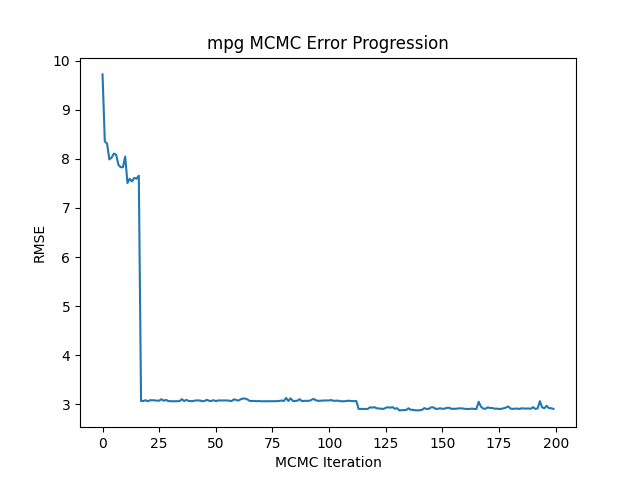
\includegraphics[scale=0.66]{mpg_phi.png}
    \caption{Typical error results for one of the datasets during the MCMC process shows burn-in achieved after about 25 iterations.}
    \label{fig:phi}
\end{figure}

For comparison to BARN, we also train a single large neural network and an equivalently sized BART forest.  For the large neural network, we retain a single hidden layer, but we set the number of neurons equal to the total neuron count in the ensemble.  Such a network necessarily has more weights than the inspiring BARN model (BARN has no direct weights between different networks), but we can quickly train it in a single pass of 200 epochs using the same optimization and regularization parameters.  Likewise, we set the number of BART trees to the same as BARN networks, 10, otherwise running with default parameters.  This already encourages small trees, and BART is fast, so a burn-in of 1000 iterations is sufficient and computable.  This provides two alternatives against which to evaluate BARN.

For each data set, we perform 13 random trials with each type of model.  We randomly split the data into 50\% training, 25\% validation, and 25\% testing (using the same split across model types for consistency) differently for each trial.  After completion, we compute the average root mean square error (RMSE) of the test predictions.  In \autoref{tab:results}, we also include the standard deviation of these results.  \autoref{fig:results} shows the average RMSE in a bar plot with error bars for a more visual comparison (though sometimes one method is so poor that it is difficult to compare the other two).

\begin{table}[htb]
\centering
\caption{Average RMSE (and standard deviation) over 13 runs of various methods on different datasets.  Smallest average error in bold.}
\begin{tabular}{lrrrr}
Dataset   &     BARN &    Big NN &      BART & OLS\\ \hline
boston    &  4.73 (0.52 )  &  7.18 (1.98 )  &  \textbf{3.99} (0.50 )  &  4.83 (0.45) \\
concrete   & 7.57 (0.55 )  & 12.68 (7.87 )  &  \textbf{6.70} (0.40)  & 10.60(0.36) \\
crimes     & \textbf{0.14 } (0.01 )  & 0.20 (0.04)  &  0.15(0.01 )  & 0.14(0.01) \\
diabetes  & 53.74(2.57)  & 53.76 (2.16)&  59.69(3.49)  & \textbf{53.67} (2.36) \\
fires     & \textbf{55.01} (39.88)  & 55.18 (39.90) &  72.28 (32.11)  & 56.46 (38.68) \\
    isotope    & 0.03  ($<$0.01)  & 0.04 (0.01)  &  0.03 ($<$0.01 )  & \textbf{0.03} ($<$0.01) \\
mpg        & 3.60 (0.48)  & 60.02 (68.58 )  &  3.50  (0.45)  & \textbf{3.33} (0.29) \\
random    & 11.16 (0.63 )  & 11.68 (0.60) &  49.72 (13.92)  & \textbf{10.02} (0.34) \\
wisconsin & \textbf{32.12} (1.73)  & 42.70(11.88 ) 0&  35.76 (3.21)  & 40.38(4.77) \\
\end{tabular}
    \label{tab:results}
\end{table}

\begin{figure}[ht]
\centering
    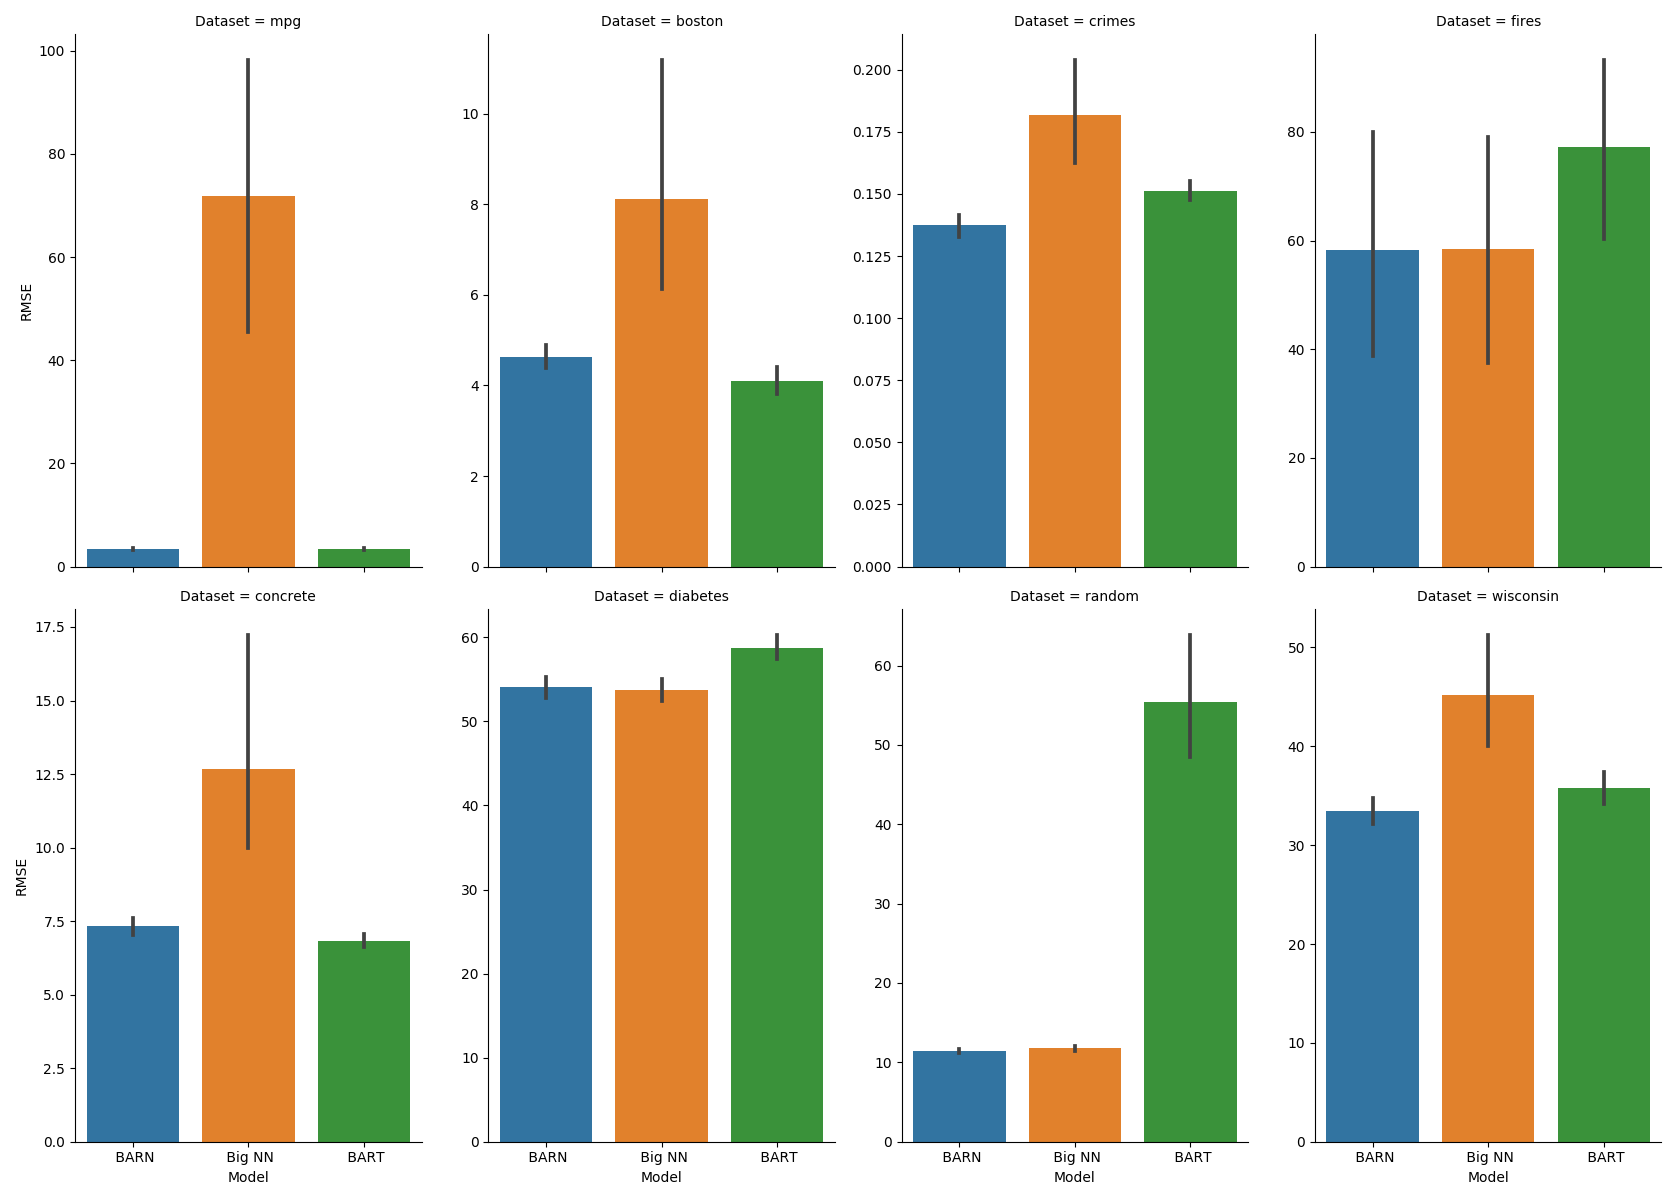
\includegraphics[scale=.3]{pres_results.png}
    \caption{BARN almost always matches or beats other methods, and is more stable}
    \label{fig:results}
\end{figure}


\subsection{Computational Costs of BARN}\label{subsec:cost}

While the previous subsections described BARN's performance in terms of error, we also consider the computational cost of running it.  An algorithm which is somewhat less accurate but much cheaper to compute still has value, especially on large data sets.  Conversely, an algorithm which provides robust results but takes significantly longer may still have applications where such stability concerns are prominent.

\autoref{tab:times} shows the mean (and standard deviation) of computation times for our various methods on the benchmark problems.  Note that we are using scikit-learn \cite{scikit-learn} with Python to perform the NN, BARN, and OLS computations (whereas BART is called from R).  Especially for neural networks, there are faster implementations available such as TensorFlow \cite{tensorflow2015whitepaper} or PyTorch \cite{paszke2019pytorch}.   Therefore we consider these measurements as preliminary.  

\begin{table}[htb]
\centering
\caption{Average training time (and standard deviation) over 13 runs of various methods on different datasets.  Note that OLS is the fastest across all dataset.}
\begin{tabular}{lrrrr}
Dataset   &     BARN &    Big NN &      BART & OLS\\ \hline
boston     & 74.20 (7.25)  & 0.10 (0.05)&  0.19 (0.03)  & $<$0.01 ($<$0.01) \\
concrete  & 131.89 (12.90)  & 0.11 (0.06)&  0.46 (0.02)  & $<$0.01 ($<$0.01) \\
crimes     & 67.58 (7.17)  & 0.11 (0.07)&  0.81 (0.06)  & 0.01 ($<$0.01) \\
diabetes  & 101.47 (6.13)  & 0.08 (0.02)&  0.15 (0.03)  & 0.01 (0.04) \\
fires      & 57.29 (10.08)  & 0.04 (0.03)&  0.14 (0.02)  & $<$0.01 ($<$0.01) \\
isotope    & 63.44 (16.40)  & 0.06 (0.01)&  0.29 (0.04)  & $<$0.01 ($<$0.01) \\
mpg        & 30.25 (2.82)  & 0.02 (0.02)&  0.14 (0.01)  & $<$0.01 ($<$0.01) \\
random    & 181.52 (16.60)  & 0.19 (0.01)&  0.49 (0.02)  & $<$0.01 ($<$0.01) \\
wisconsin  & 38.43 (3.14)  & 0.04 (0.03)&  0.09 ($<$0.01)  & $<$0.01 ($<$0.01) \\
\end{tabular}
    \label{tab:times}
\end{table}


Based on the current implementation, we see that BARN is significantly slower than all of the other methods tested.  Note, however, that the equivalently sized neural network is not nearly as slow (about 1000x faster than BARN).  Part of this is that BARN has to train networks many times (i.e. the burn in period plus the sampling period, 200 iterations in this study).  But part of this cost is also constantly loading/unloading BARN's NNs into memory (as stored by scikit-learn).

These observations suggest two possible speedups.  First, an implementation in TensorFlow could take advantage of Graphical Processing Units (GPUs), enabling a high level of parallelism for the NN training process.  This parallelism can provide an immediate 5x improvement or better in computation time \cite{lind2019performance}.  Next, the memory loading/unloading operations could be minimized by storing the many small NNs of BARN as one large NN.  That is, keep the overall neuron count, but zero out weights that represent ``cross-NN'' connections.  Further, when training, one can mask off only the relevant components for updating during backpropagation.  This does require some careful programming, as it requires reloading the model with additional available neurons should all of them be in use yet the MCMC process proposes adding a new one to a model.  But this would bypass most of the loading time, further decreasing the overall computation time.

\subsection{BARN and clumped isotope paleothermometry}\label{subsec:therm}

In addition to the benchmark data sets, we also apply BARN to a recent problem in clumped isotope paleothermometry.  A recent study \cite{roman2022bayclump} demonstrated the effectiveness of a Bayesian least squares approach to this data.  Such a method uses a linear model as in OLS, but uses priors on the estimated parameter values informed by earlier studies.  BARN also uses priors but on the model structure (by affecting the size of learned networks) rather than the parameters directly.  An interesting future study might add priors on model weights in BARN as well, but we run standard BARN on this data for now.

The modeling problem itself is to predict carbonate clumped isotope thermometry, $\Delta_{47}$, as a function of temperature \cite{eiler200418o13c16o}.  This is a calibration process; in practice one uses $\Delta_{47}$ as a surrogate for temperature.  The ecological details are beyond the scope of this paper, but there are various studies on this topic \cite{eiler200418o13c16o,roman2022bayclump,petersen2019effects}.

From \autoref{tab:results} and \autoref{fig:results} under the ``isotope'' data set, we can see that BARN performs well relative to the other methods we test.  In this case, the lowest error model is OLS, but only by a marginal amount.  BARN produces very similar results to OLS (albeit at a greatly increased computational cost).  It may be that the structural model of a neural network tends to reduce to an OLS-like result in this situation with a single explanatory varaible.

Note that in other Bayesian linear models \cite{roman2022bayclump}, the testing error across methods is similar to OLS.  \autoref{fig:iso_results} combines these with our methods for this specific data set for easy comparison.  In particular, BARN appears to be in the same class of error levels as the best linear approaches.  This is especially interesting because the other nonlinear methods we tested (the big NN and BART) actually perform significantly \emph{worse} than OLS (and BARN).  It is possible that BARN is able to simplify to an OLS-like model that is appropriate for this problem (which has a single explanatory variable) where other nonlinear methods would require additional training data for such a reduction.  This demonstrates the adaptability and broad applicability of BARN.

\begin{figure}[ht]
\centering
    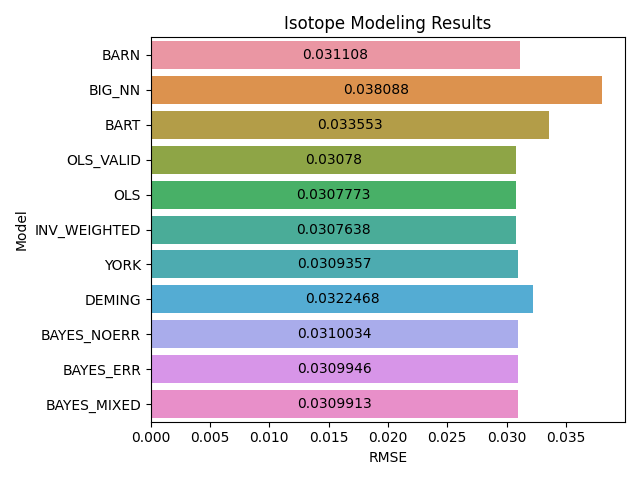
\includegraphics[scale=.7]{iso_results.png}
    \caption{RMSE on D47 testing data for various methods.  BARN performs similarly to linear methods \cite{roman2022bayclump} even when a big NN and BART perform significantly worse.  Note that methods used in this study (top four models) reserve 25\% of the training data for validation (hence why ``OLS\_VALID'' is separate from ``OLS'').}
    \label{fig:iso_results}
\end{figure}



\section{Discussion}\label{sec:dis}

Based on \autoref{tab:results} and \autoref{fig:results}, BARN is competitive with both single hidden layer neural networks and BART for most data sets.  Note that we recompute BART results rather than using those in \cite{biau2019neural} as that used far more trees.  Particularly, BARN avoids catastrophic failures of the other methods (e.g. large Neural Network for mpg data or BART with the random linear problem).  Additionally, it is generally consistent; in those problems where it is not the most accurate, it is very close to the smallest in magnitude.  In the wisconsin data, BARN seems to be significantly better than the next best BART, even at this prototype scale.  On other problems, BARN has a lower average RMSE, but this falls within expected errors for one of the other methods (note that Neural Random Forests only have this type of improvement \cite{biau2019neural}).  And the isotope data studied shows that BARN is competitive with some of the latest bayesian linear models \cite{roman2022bayclump}, even when other nonlinear approaches perform poorly.  So although BARN is not universally superior, there are situations in which it noticeably outperforms existing methods and may be more generally robust.

This performance, however, comes at a cost.  While BART and a single NN can be trained in a few to tens of seconds, performing 200 iterations of BARN takes several minutes on these problems.  This may be in part due to implementation details; we use the Scikit-Learn Python module to handle NN training \cite{scikit-learn} and manually code the MCMC procedure.  This means each small network has to be loaded into memory, and we are not taking advantage of GPU capabilities.  Regardless, on the scale of problems considered, BARN even as a prototype was sufficiently fast.

\section{Future Work}\label{sec:future}

Though \autoref{sec:eval} shows BARN to be competitive, there remains a significant amount of future work on better theoretical understanding and practical implementation.  Most of the theoretical advances relate to more rigorous analysis of the MCMC components.  For example, our selection of transition probabilities was somewhat arbitrary, while Bayesian CART \cite{chipman1998bayesian} claimed to justify (though not explicitly state) their expressions.  We may be able to derive a tilted distribution to improve convergence and reduce variance in the produced models.  Similarly, we need better justification for our model size prior, $\lambda$.  While some kind of Poisson or Negative Binomial model is probably sufficient, a heuristic to guide the prior would be helpful.  In BART \cite{chipman2010bart}, they find tree size parameters that they claim are broadly applicable; it may be that we can find something similar for neural networks.  Finally, we assumed the residuals for each model are i.i.d normal, but this is problem dependent.  One can account for relaxations to this by modifying the $P(Y|X,M)$ expression, but it is not clear if we can derive a closed form for this similar to that of BART.  We believe our theoretical approach is sound and confirmed by the experimental results, but this remains an open area of research.

On the applied side, there is also fruitful future research.  Our results are for small-scale ensembles of only 10 NNs, but to take more inspiration from BART, we suspect on the order of 100 NNs will be more effective.  Likewise, a larger ensemble may require a longer burn-in period (BART uses 1000 by default \cite{chipman2010bart}).  Each of these changes comes with a direct cost of 10 times as much computation, however, so we may first consider writing more computationally efficient software.  TensorFlow with Keras \cite{chollet2015keras} can provide a straightforward GPU-capable library for building the component neural networks.  Further, we may be able to better cache intermediate results, possibly by storing the ensemble in one large network.  We can create an NN with the sum of the neuron counts similar to our comparison in \autoref{sec:eval}, but then zero the weights on what would be cross network connections.  And when running the model, we could mask off entire unused neurons (i.e. preload a network with say 100 neurons, but only unmask them as needed).  These improvements may also enable BARN to address larger scale problems like age estimation from facial images or other big data problems.

Such problems naturally suggest additional types of models to implement in BARN.  In the vein of deep learning, we may want to enable multiple hidden layers of neurons.  Or for image data, it may be helpful to have a convolutional layer architecture (computing the same filter on different regions of an image).  These types of changes, however, require a mechanism for transitioning between states (e.g. when adding a new layer, do we add a single neuron, or several?).  Bayesian CART \cite{chipman1998bayesian} notes that this can be difficult to derive (though it may still be feasible to specify something, even if not optimal).  Broadening our view further, we can also extend BARN to classification tasks.  Researchers have recently expanded BART to multinomial logistic (rather than probit) outcomes \cite{xu2021inference}; we should be able to apply that technique to BARN if not adapt the additive regressors directly to the various logit estimations (essentially aggregating the residuals into the logit bias terms).  The most general view, however, would be to apply this BART/BARN approach to \emph{any} model type.  So long as one can specify the MH components: a model transition probability, $q(M,M')$, a model fit likelihood, $P(R_k|X, M')$, and a model prior probability, $P(M')$, this approach should be feasible.  This would be fruitful to study more theoretically and empirically with a variety of model types.  As a generalization of BART, BARN has many new research possibilities.

\section{Conclusions}

We introduce and demonstrate the effectiveness of a new model ensemble technique, Bayesian Additive Regression Networks.  This approach adapts the bayesian MCMC method of BART to neural networks rather than decision trees.  On a variety of benchmark problems, BARN often outperformed competing methods and always avoided catastrophic failures.  On a more recent data set of interest, BARN compared well to other methods, even when nonlinear approaches failed.  Though highly accurate, BARN is, however, computationally expensive in its current prototype state.  Future implementations should focus on addressing this and generalizing BARN further to other types of neural networks or generic models.

\clearpage

\bibliography{lib}

\end{document}
